what is this chapter about
how is evaluation perfromed
our shader
evaluation java table generator provided by daljit.
explain how this program works:
subvariants: sample whole lambda space, just a few lambdas, pq approach.
how from those generated tables to matlab
how to read those
discussion


\chapter{Evaluation Data Acquisition}
\section{Data Acquisition}
For measurement on the true surface topography of snake sheds, samples are stuck on glass plates using double face tape, the animal was pushed up below a hollowed plate letting the skin emerging from the top of the plate. the surface of the scale under measurement should be large compared to the size of the drop to avoid wetting the plasmic membrane that would corrupt the reasing of the contact angle. 

Measurements were carried out using intermittent contact mode in a Burker Dimension 3100 atomic force microscope (AFM) under ambient conditions using a Nanoscope V controller. 

An AFM is a microscope that uses a tiny probe mounted on a cantilever to scan the surface of an object. The probe is extremely close tobut does not touchthe surface. As the probe traverses the surface, attractive and repulsive forces arising between it and the atoms on the surface induce forces on the probe that bend the cantilever. The amount of bending is measured and recorded, providing a map of the atoms on the surface. Atomic force microscopes can achieve magnification of a factor of 5 × 106, with a resolution of 2 angstroms, sufficient to resolve individual carbon atoms. Also called scanning force microscope.
is a very high-resolution type of scanning probe microscopy, with demonstrated resolution on the order of fractions of a nanometer, more than 1000 times better than the optical diffraction limit.

The tops used were etched silicon TESP tips with a nominal frequency and force constant of 320 kHz and 42 N/m respectively. 

SHOW AFM IMAGE

\section{Diffraction Gratings}
An idealised grating is made of a very large number of parallel, evenly spaced slits in an in an opaque sheet. Typically, it would have about 10,000 slits. In order to cause diffraction, the spacing between slits must be wider than the wavelength of interest. Each slit in the grating acts as a quasi point source from which light propagates in all directions. The diffracted light is composed of the sum of interfering wave components emanating from each slit in the grating.

\begin{figure}[ht]
  \centering
  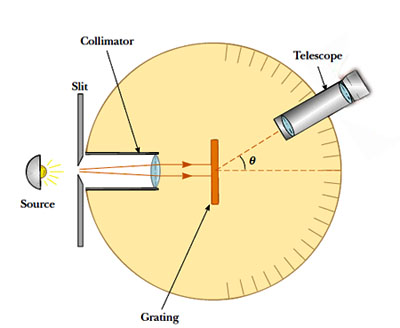
\includegraphics[scale=0.7]{evaluation/spectrometer.jpg}
  \label{fig:spectometer}
  \caption{Spectometer: When a beam of monochromatic light passes through a grating placed in a spectrometer, images of the sources can be seen through the telescope at different angles.}
\end{figure}

Suppose monochromatic light is directed at the grating parallel to its axis as shown in figure. Let the distance between successive slits be equal $d$.

\begin{figure}[ht]
  \centering
  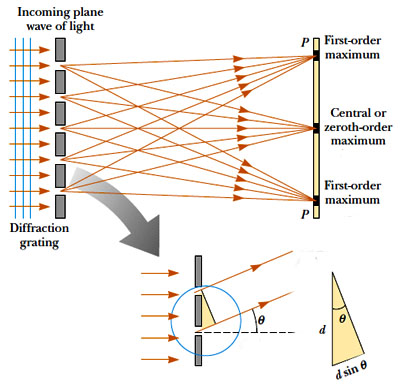
\includegraphics[scale=0.7]{evaluation/grating2.jpg}
  \label{fig:lighthitsgrating}
  \caption{Light directed to parallel to grating:}
\end{figure}

The diffraction pattern on the screen is the result of the combined effects of diffraction and interference. Each slit causes diffraction, and the diffracted beams in turn interfere with one another to produce the pattern. The path difference between waves from any two adjacent slits can be found by dropping a perpendicular line between the parallel waves. By geometry, this path difference is $d sin(\theta)$. If the path difference equals one wavelength or some integral multiple of a wavelength, waves from all slits will be in phase and a bright line will be observed at that point. Therefore, the condition for maxima in the interference pattern at the angle $\theta$ is: 

\begin{equation}
 d sin(\theta) = m \lambda 
\end{equation}

where $m \in \mathds{N}_0$ is the order of diffraction.

Because $d$ is very small for a diffraction grating, a beam of monochromatic light passing through a diffraction grating is splitted into very narrow bright fringes at large angles $\theta$.

\begin{figure}[ht]
  \centering
  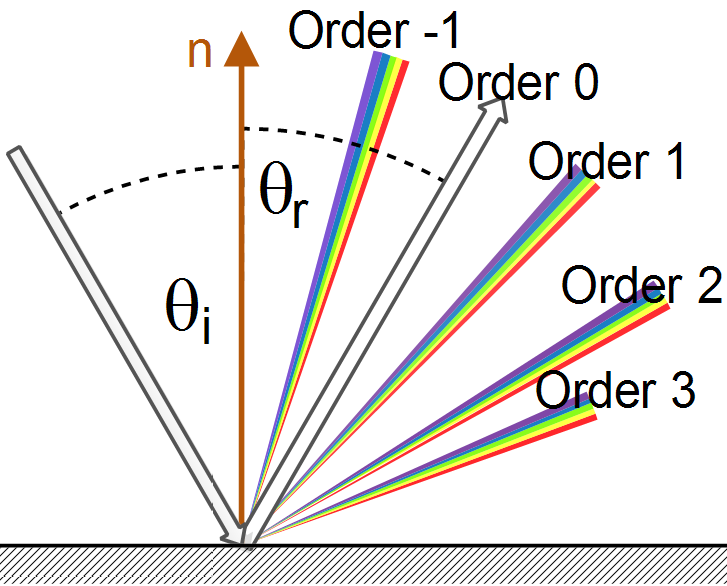
\includegraphics[scale=0.7]{evaluation/GratingSurface.png}
  \caption{Different Orders of diffraction: When light is directed at the grating not parallel to its axis, there is another $sin(a)$ invovled. See grating equation $\ref{eq:gratingEq}$.}
\label{fig:gratingdiffractionorders}
\end{figure}

When a narrow beam of white light is directed at a diffraction grating along its axis, instead of a monochromatic bright fringe, a set of coloured spectra are observed on both sides of the central white band as shown in figure $\ref{fig:gratingdiffractionorders}$.

\begin{figure}[ht]
  \centering
  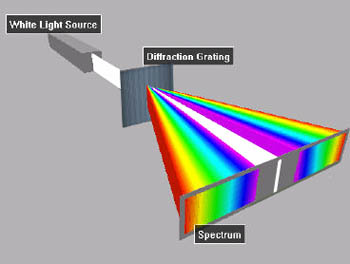
\includegraphics[scale=0.7]{evaluation/coloredspectrum.jpg}
  \label{fig:diffractionSpectrum}
  \caption{White Light beam causes coloured diffraction spectra}
\end{figure}

Since $\theta$ increases with wavelength $\lambda$, red light which has the longest wavelength is diffracted through the largest angle. Violet light has the shortest wavelength and is diffracted the least. Thus, white light is split into its component colours from violet to red light. The spectrum is repeated in the different orders of diffraction. Only the zeroth order spectrum is pure white.

\begin{figure}[ht]
  \centering
  \subfigure[one slits]{
    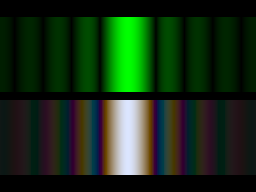
\includegraphics[scale=0.1]{evaluation/slits/spalt1.png}
    \label{fig:diffractionSlits1}
  }
~
  \subfigure[two slits]{
    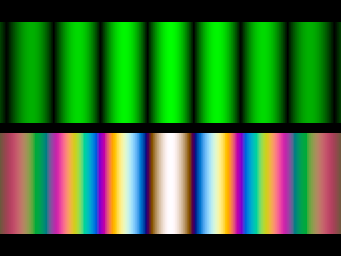
\includegraphics[scale=0.1]{evaluation/slits/spalt02.png}
    \label{fig:diffractionSlits2}
  }
~
  \subfigure[three slits]{
    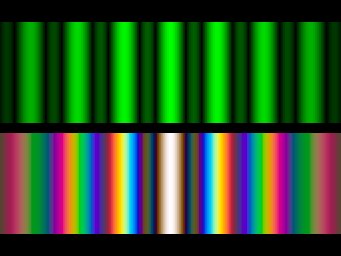
\includegraphics[scale=0.1]{evaluation/slits/spalt03.png}
    \label{fig:diffractionSlits3}
  }
~
  \subfigure[seven slits]{
    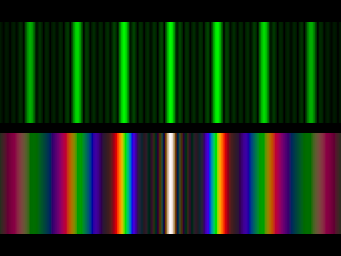
\includegraphics[scale=0.1]{evaluation/slits/spalt07.png}
    \label{fig:diffractionSlits7}
  }
  
  \label{fig:diffractionSlits}
  \caption{Difference of diffraction pattern between a monochromatic (top) and a white (bottom) light spectra for different number of slits.}
\end{figure}


WHITEMONODIFF
The figure below shows the di.


\section{Evaluation}
UNIFY ANGLE NAMES: 

In order to check the physical reliability of our method we applied it on a syntetic blazed grating, Elaphe and Xenopeltis snake sheds and evaluated its response using the grating equation. This equation models the relationship between the grating spacing and the angles of the incident and diffracted beams of light. 

When light at a wavelength $\lambda$ falls on a sample presenting a periodicity $d$ along the incident plane under an incident angle $\theta$ compared to the normal of the surface the angle $\phi$ corresponding to the direction of the emerging beam showing constructive interferences (maximum in intensity) is given by the grating equation:

\begin{equation}
  sin(\theta) = sin(\phi) + \frac{m \lambda}{d}
  \label{eq:gratingEq}
\end{equation}

In our evaluation we are interested in the zero order diffraction, i.e. m equals zero which corresponds to direct transmission or specular reflection in the case of a reflection grating. 
Within our evaluation we further assume that the incident light direction $w_i$ is given. In contrast the direction of the reflected wave $w_r$ is not given.
In Mathematics, a three dimensional direction vector is fully defined by two two angles, i.e. it can be represented by spherical coordinates with radius $r = 1$. By convention, we denote those two vectors by $\theta$ and $\phi$. Hence, $\theta_i$, $\phi_i$ and $\phi_r$ are given constants whereas $\theta_i$ is a free parameter for our evaluation simulation. Therefore, we are going to compare the maxima for peak viewing angle corresponding to each wavelength using data produced by our method against the maxima resulting by the grating equation.

\subsection{Precomputation}
SHOW IMAGE OF GRID

Before being able to compare the output produced by our method by the grating equation, we have to discretise the wavelength space $\Lambda$ and the range $\Theta$ of our free parameter $\theta_i$. We also have to initially assign  $\theta_i$, $\phi_i$ and $\phi_r$. For our experiments we choose the following initial setup: $\theta_i = 75$ $\phi_i = 0$ $\phi_r = 180$ degree.
Further we discretise the lambda space $\Lambda = \{\lambda | \lambda = \lambda_{min} + k\lambda_{step}, k \in \{0,..,C-1\}\}$ where $\lambda_{step} = \frac{\lambda_{max}-\lambda_{min}}{C-1}$ and $C$ is the discretisation level of the lambda space, in our scenario $C = 42$. We similarly discretise the angle space by predefining an minimal and maximal angle boundary and $ceil(angMax - angMin) / angInc$ is the number of angles. 
We are going implement a similar algorithm as the diffraction fragment shader algorithme on the grid $[\Lambda, \Theta]$ and will store its spectral response in a matrix $R = \{response(\lambda_i, \theta_{r}^{j}) | i index(\Lambda), j index(\Theta)\}$. We also have evaluated our other shaders, mentioned within the discussion of the derivation and implementation chapters.

\subsection{Data evaluation}

\begin{algorithm}
\caption{Evaluation: lambda thetar graph}
\label{alg:evalmatlab}
\begin{lstlisting}
% load all variables computed in java
lInc = (lMax - lMin)./(lambdaCnt-1);
lambda = lMin + lInc*(-1+[1:lambdaCnt]);
[maxC maxI] = max(response.');
viewAngForMax = angMin + angInc * (maxI-1);
plot(lambda, viewAngForMax,'-r');s

for thetaI=baseAngle-eps:0.5:baseAngle+eps,
	% grating equation
	thetaV = asin(lambda./dPeriod - sin(thetaI*pi()/180))*180/pi();
	if(thetaI==75)
		plot(lambda, thetaV,'+ b');
	else
		plot(lambda, thetaV,'. g');
	end
end

\end{lstlisting}
\end{algorithm}

\begin{figure}[ht]
  \centering
  \subfigure[plot $\lambda$ - $\theta_i$]{
    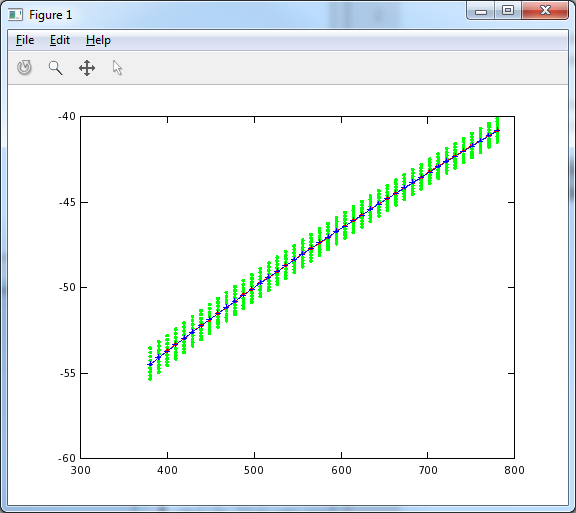
\includegraphics[scale=0.19]{blaze2500_75.png}
    \label{fig:evalBlaze11}
  }
~
  \subfigure[Zoomed in]{
    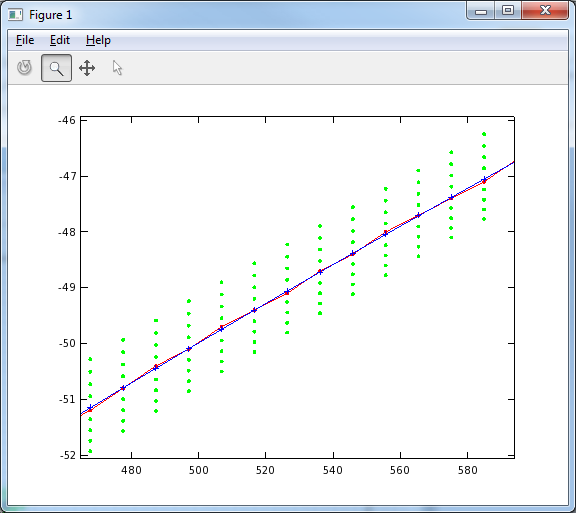
\includegraphics[scale=0.19]{blaze2500_75_closeup1.png}
    \label{fig:evalBlaze12}
  }
~
\subfigure[Further zoomed in]{
  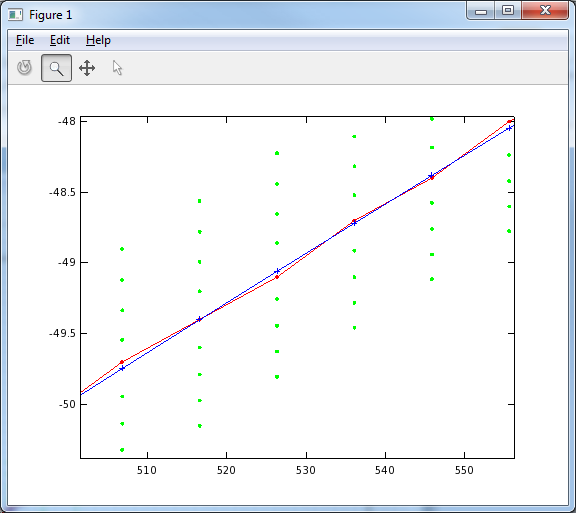
\includegraphics[scale=0.19]{blaze2500_75_closeup2.png}
  \label{fig:evalBlaze13}
}
  \label{evaluationBlaze1}
  \caption{Evaluation: blaze grating}
\end{figure}

red graph is based on data produced by our method, the blue and green graphs are plots from the grating equation for different angles. If the blue graph is close the the red one, then our method performs well. 

SHOW PLOTS AND TALK ABOUT THEM
